\documentclass[a4paper,oneside]{mystyle}
\usepackage[utf8]{inputenc}

% custom packages
\usepackage{empheq}
\usepackage{graphicx}
\usepackage[font={small}]{caption}
\usepackage{subcaption}
\usepackage{framed}
\usepackage{listings}
\usepackage{wrapfig}
\usepackage{sidecap}
\usepackage{xcolor}
\usepackage{lineno}
\usepackage{marvosym}
\usepackage{xstring}
\usepackage{mfirstuc}
\usepackage{pdfpages}
\usepackage{lipsum}
\usepackage[explicit]{titlesec}
\usepackage{cancel}
\usepackage[noabbrev]{cleveref}


%%%%%%%%%%%%%%%%%%%%%%%%%%%%%%%%%%%%%%%%%%%%%%%%%%%%%%%%%%%%%%%%%%%%%
% DOCUMENT METADATA

\thesistype{Master thesis}
\title{ProSLAM student edition: a minimalistic stereo visual SLAM system}

\author{Irvin Aloise}
\email{aloise.1392066@studenti.uniroma1.it}
\institute{RoCoCo - Cognitive robot teams laboratory\\[2pt]
Department of Computer, Control and Management Engineering Antonio Ruberti\\[2pt]
Sapienza University of Rome}

\supervisors{Prof.\ Dr.\ Giorgio Grisetti}
\cosupervisors{Eng.\ Dominik Schlegel}

\date{\today}

%%%%%%%%%%%%%%%%%%%%%%%%%%%%%%%%%%%%%%%%%%%%%%%%%%%%
\lstset { %
	language=C++,
	backgroundcolor=\color{black!5}, % set backgroundcolor
	basicstyle=\footnotesize,% basic font setting
}


%ds colors
\definecolor{orange}{rgb}{1,0.4,0}
\definecolor{green}{rgb}{0,0.5,0}

%ds referencing
\newcommand{\myref}[3]{\hyperref[#1]{#2} (\capitalisewords{#3} \ref{#1})}

%ds blue box
\definecolor{myblue}{rgb}{.9, .9, 1}

\newlength\mytemplen
\newsavebox\mytempbox
\newcommand*\widefbox[1]{\fbox{\hspace{2em}#1\hspace{2em}}}

\makeatletter
\newcommand\mybluebox{%
	\@ifnextchar[%]
	{\@mybluebox}%
	{\@mybluebox[0pt]}}

\def\@mybluebox[#1]{%
	\@ifnextchar[%]
	{\@@mybluebox[#1]}%
	{\@@mybluebox[#1][0pt]}}

\def\@@mybluebox[#1][#2]#3{
	\sbox\mytempbox{#3}%
	\mytemplen\ht\mytempbox
	\advance\mytemplen #1\relax
	\ht\mytempbox\mytemplen
	\mytemplen\dp\mytempbox
	\advance\mytemplen #2\relax
	\dp\mytempbox\mytemplen
	\colorbox{myblue}{\hspace{1em}\usebox{\mytempbox}\hspace{1em}}}

%ds global definitions
\def\P{\mathcal P}
\def\tab{\phantom{tab}}
\def\homx{\mathbf{\tilde{x}}}
\def\trans{\mathbf{t}}
\def\quat{\mathbf{q}}
\def\state{\mathbf{x}}
\def\meas{\mathbf{z}}
\def\error{\mathbf{e}}
\def\jacob{\mathbf{J}}
\def\kdtree{\textit{K}-D tree}
\def\T#1#2{^{#1}T_{#2}}
\def\t2v#1#2{^{#1}\tau_{#2}}
\def\deltat2v#1#2{^{#1}\Delta\tau_{#2}}
\def\chref#1{Chapter~\ref{ch:#1}}
\def\secref#1{Sec.~\ref{#1}}
\def\figref#1{Fig.~\ref{#1}}
\def\tabref#1{Tab.~\ref{#1}}
\def\eqref#1{Eq.~(\ref{#1})}
\def\algref#1{Alg.~\ref{#1}}
\def\lstref#1{Lst.~\ref{#1}}
\def\ourmethod{\textit{g2o\_slim~}}
\renewcommand{\thesubfigure}{\Alph{subfigure}}


\begin{document}
	
\frontmatter
\begin{titlepage}
\maketitle
\cleardoublepage\null
\thispagestyle{empty}
\end{titlepage}

\newcounter{notation}
\begin{abstract}
The goal of this Master's Thesis is the design and development of a graph-optimization system tailored for SLAM pipelines. The work focuses on simplicity, accuracy and speed, reaching excellent results in each of the targeted fields.

In particular, this back-end aims attention at 3D pose-graphs and 3D pose-landmark problems, producing outcomes comparable to current state-of-the-art systems like \texttt{g2o} \cite{kummerle2011g}. 

At its core there is a novel error function for $SE(3)$ objects based on the concept of matrices' chordal distance. This approach reduces the problem's non-linearity bringing several benefits to the computation. The fastness of the system is due to a well-designed implementation that performs zero memory copy during the iterative part and that exploits SIMD instructions of modern CPUs and a smart use of the CPU cache.

Finally, the system has been tested on both synthetic and real-world datasets and in both scenarios it succeeded in its purposes, being able to produce results better or comparable to state-of-the-art systems in only 5 thousands lines of code. 
\end{abstract}

\chapter*{Nomenclature}\label{ch:symbols}
\addcontentsline{toc}{chapter}{Nomenclature}

\section*{Notation}
\refstepcounter{notation}
\label{sec:notation}

\begin{tabbing}
	\hspace*{3.0cm}		\= \kill
	$^A\rot_{B}(\alpha, \beta, \gamma)$ \> Rotation from frame A to frame B expressed in A \\[0.75ex]
	$^A\trans_{B}(t_x,t_y,t_z)$ \> Translation from frame A to frame B expressed in A  \\[0.75ex]
	$\T{A}{B}(R,\trans)$ \> Transformation from frame A to B expressed in A  \\[0.75ex]
	$\t2v{A}{B}(R,\trans)$ \> Transformation from frame A to B expressed in A (vectorized) \\[0.75ex]
	${\lfloor\trans\rfloor}_\times$ \> Skew-symmetric matrix of a vector $\mathbf{t} \in \mathbb{R}^{3\times3}$
\end{tabbing}

\section*{Acronyms and Abbreviations}
\label{sec:acronyms}
\begin{tabbing}
	\hspace*{3.5cm}		\= \kill
	SLAM \> Simultaneous localization and mapping \\[1ex]
    SfM \> Structure from Motion \\[1ex]
    BA \> Bundle Adjustment \\[1ex]
    SCLAM \> Simultaneous Calibration Localization and Mapping \\[1ex]
    MAP \> Maximum A Posteriori \\[1ex]
    LS \> Least Squares \\[1ex]
    PSD \> Positive Semi-Definite \\[1ex]
    PDF \> Probability Distribution Function \\[1ex]
    Landmark \> Salient point in the world (2D or 3D) \\[1ex]
	Feature \> Specific structural part of interest in an image (2D) \\[1ex]
	Tracking \> Procedure of spatial and temporal re-identification of landmarks \\[1ex]
	Loop closure \> Interconnection between landmarks in space \\[1ex]
	GPS \> Global Positioning System (generally referring to whole unit) \\[1ex]
    LiDAR \> Light Detection and Ranging o Laser Imaging Detection and Ranging \\[1ex]
    Sonar \> SOund Navigation And Ranging \\[1ex]
    FLOP \> Floating Point OPeration \\[1ex]
    FLOPS \> Floating Point Operations Per Second \\[1ex]
	OpenCV  \> Open source Computer Vision (library), \url{www.opencv.org} \\[1ex]
	Git  \> Git revision control, \url{www.git-scm.com} \\[1ex]
\end{tabbing}

\clearpage

\tableofcontents
\mainmatter
\newpage
\chapter{Introduction}\label{ch:intro}
Mobile robots, in order to accomplish tasks in real world more easily and in an efficient way, need to have a map of the environment and to localize themselves into the map. Furthermore, in some environment it is not possible to rely on external reference systems - e.g. GPS - and, thus, they can count only on on-board sensors. \textit{Simultaneous Localization and Mapping} (SLAM) addresses the problem of \textbf{learning the map under pose uncertainty}.

There are many scenarios in which SLAM is fundamental for the accomplishment of a task, not only in pure Robotics. SLAM, in fact, is a common problem in different domains of application. For example, in Robotics it is fundamental for indoor navigation of mobile robots - e.g. an autonomous vacuum cleaner or a service robot in a museum - or to navigate through extreme environments - e.g. underwater rescues or space exploration. Additionally, new technologies that involve different kind of agents - i.e. not robots - are now using SLAM. One of the most trending is \textit{Augmented Reality} (AR). Always more powerful mobile devices - like smartphones or tablets - are now able to exploit SLAM to deliver stunning virtual experiences. Without any doubts, this technology is going to gain always more popularity and to impact on the research in this topic.
\vspace{5px}

\begin{figure}[!hbt]
    \centering
    \begin{minipage}[t!]{0.4\textwidth}
        \centering
        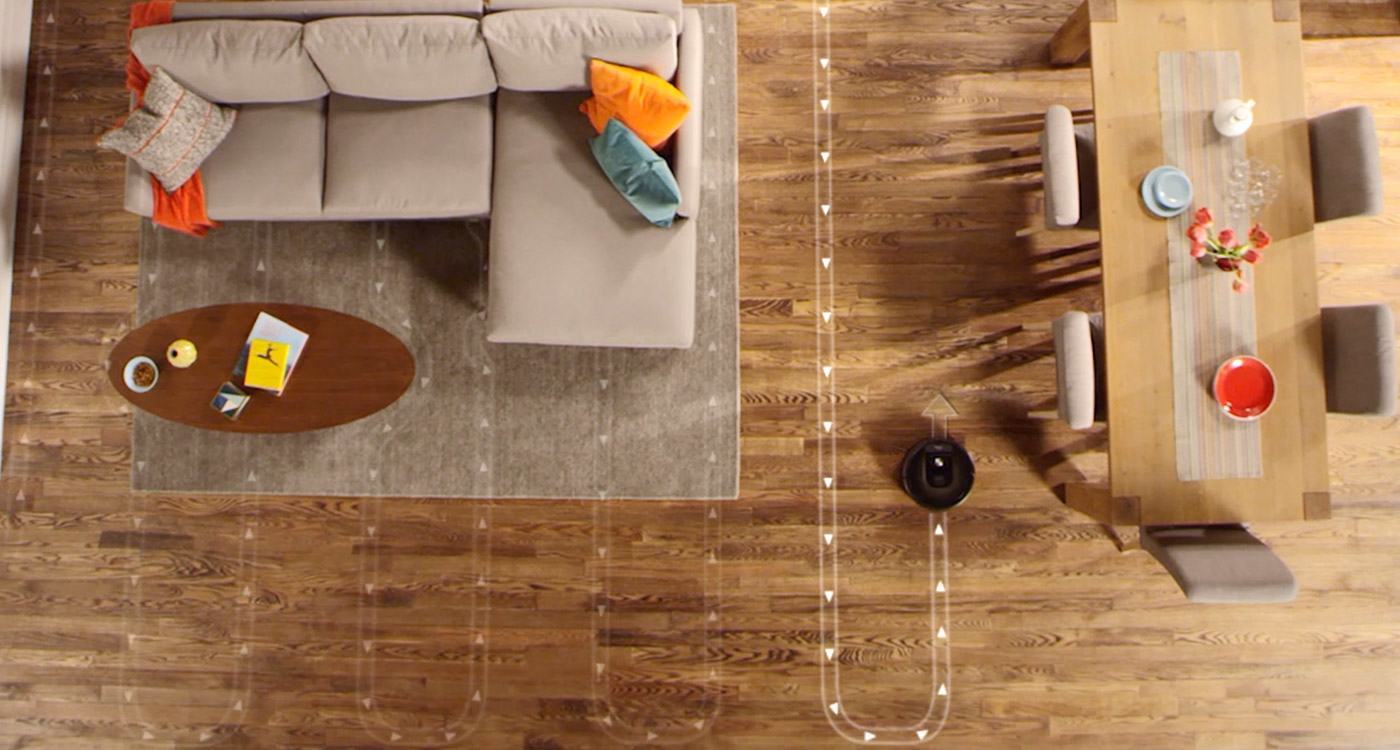
\includegraphics[width=\textwidth]{figures/00_intro/roomba_cleaning.jpg}
        \subcaption[first caption.]{}
        \label{fig:roomba}
    \end{minipage} \hspace{10px}
    \begin{minipage}[t!]{0.4\textwidth}
        \centering
        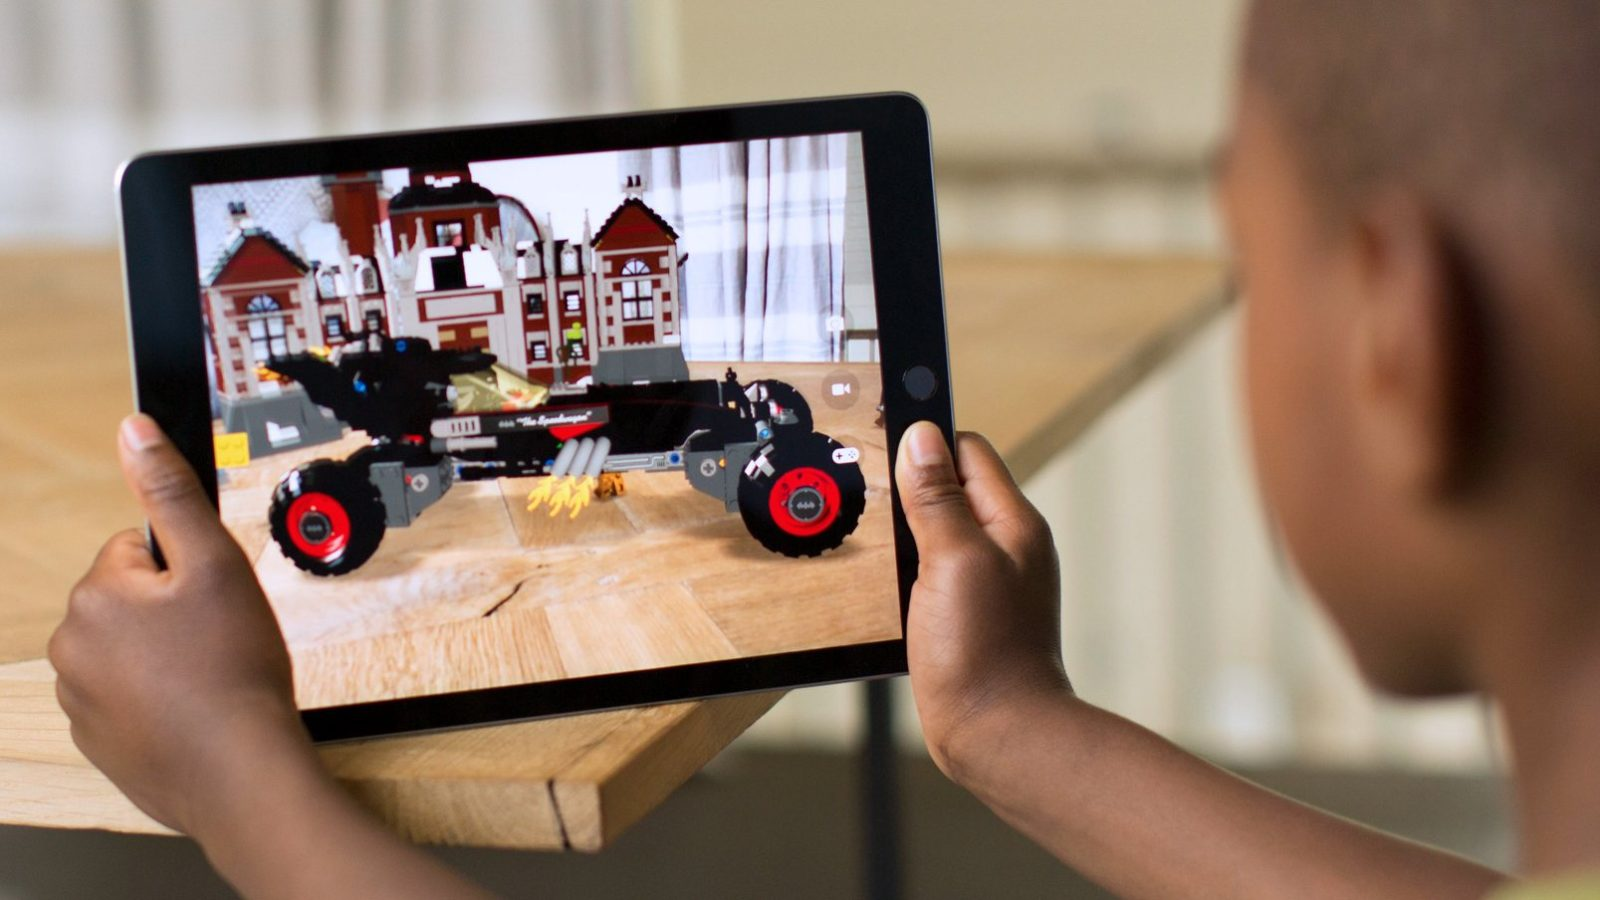
\includegraphics[width=\textwidth]{figures/00_intro/apple_ARKit.jpg}
        \subcaption[second caption.]{}
        \label{fig:apple_ARKit}
    \end{minipage}%
    
    \caption{\textbf{Application Examples.} The image in \ref{fig:roomba} represents the well-known Roomba Autonomous vacuum cleaner, which is able to recognize where it is in the room, if it has already cleaned a place or if it is going toward a dangerous path - e.g. stairs; image \ref{fig:apple_ARKit} depicts an AR mobile game developed using the Apple ARKit.} 
    \label{fig:applications}
\end{figure}

As the reader might notice, SLAM is a popular problem and the research community is focusing on it since many years. Several solutions have been proposed through the years and now current state-of-the-art SLAM systems are able to deliver impressive results in real-world scenarios. The most used formulation for the SLAM problem is the so-called \textit{graph-based SLAM}. In this approach, two sub-systems cooperate with each other to retrieve the best robot trajectory and world configuration given the on-board sensors' measurements. Therefore, the full slam system is composed by:

\begin{enumerate}
    \item \textit{Front-end}: it exploits sensor data to build an hyper-graph whose nodes are either robot poses or the position of salient points in the world;
    \item \textit{Back-end}: it is in charge of performing non-linear optimization of the graph to retrieve the most likely configuration that suits the measurements.
\end{enumerate}

In this work, we propose a back-end system built from scratch that is able to perform fast and accurate graph optimization for 3D environments. The work is focused on simplicity and minimalism also in its implementation, in order to be comprehensible by non-expert people that what to understand how the system works. Despite its minimalistic fashion, system's results are comparable - or even better in some scenarios - to the ones of other state-of-the-art systems, thanks to the use of some novel theoretic ideas and to a well-designed implementation. In particular, this work shows the effectiveness of a \textbf{new error function} for $SE(3)$ objects (Section \ref{sec:se3_objects}) and an implementation with \textbf{zero memory copy} during the optimization process (Section \ref{sec:bottlenecks}).

\vspace{20px}

\noindent The remaining of this document is organized as follows:

\begin{itemize}
    \item Chapter \ref{ch:related}: overview of the problem and of methodologies employed through the years, with a particular focus on noteworthy systems;
    \item Chapter \ref{ch:basics}: problem statement and fundamental theoretic concepts related to the non-linear optimization problem;
    \item Chapter \ref{ch:problems}: sketch of the most common SLAM problem formulations;
    \item Chapter \ref{ch:solvingSE3}: deeper examination of 3D formulations and further analysis of the proposed approach;
    \item Chapter \ref{ch:implementation}: details about code design and implementation choices;
    \item Chapter \ref{ch:cases}: focus on two full SLAM systems that uses the proposed system as on-line back-end;
    \item Chapter \ref{ch:conclusions}: final considerations and possible future investigations. 
\end{itemize}
\newpage
\chapter{State of the Art}\label{ch:related}
\lipsum

\lipsum

\newpage
\chapter{Conclusions}\label{ch:conclusions}
\lipsum

\newpage
\bibliographystyle{splncs}
\bibliography{references}


%add appendix for dataset class
\end{document}